\documentclass[12pt,fleqn]{article}\usepackage{../../common}
\begin{document}
Uzun Kısa-Vade Hafıza Ağları (Long Short-Term Memory Networks, LSTM)

Kendini tekrarlayan YSA (RNN) yapılarının içindeki gizli konum $h_t$
(önceki yazıda $s_t$) olarak bir zaman diliminden bir diğerine
aktarılabiliyordu, ve bu sırada bir matris çarpımı üzerinden değişime
uğrayabiliyordu. Böylece her zaman diliminde yeni görülen verinin
``hafıza'' olarak ta tanımlanabilen $h_t$'ye etkisi olabiliyordu. RNN dış
dünya hakkındaki iç modelini böyle güncelliyordu.

Fakat RNN ile tarif edilen bu güncellemeye hiç bir sınır getirmedik. Biraz
düşünürsek bu güncellemenin biraz kaotik bir hal alabileceğini görebiliriz
[1]. Mesela bir filmi kare kare izleyerek filmde neler olduğunu tarif
etmeye uğraşan bir RNN düşünelim. Bir karede bir karakterin ABD'de olduğunu
düşünebilir, ama sonraki karede karakterin suşi yediğini görüyor ve
Japonya'da olduğuna karar verebilir, sonra Panda ayısı görüyor ve karakteri
kuzey kutbunda zannediyor.

Bu tarif edilen kaos enformasyonun çok hızlı etki ettiğini ve aynı hızda
yokolduğuna işaret. Bu tür bir yapıda modelin uzun vadeli hafıza tutması
oldukça zor. Bize gereken modelin sadece güncelleme yapması değil,
güncelleme yapmayı da öğrenmesi. Ali adlı bir karakter film karesinde yoksa
o kareler Ali hakkındaki bilgiyi güncellemek için kullanılmamalı, aynı
şekilde Ayşe'nin içinde olmadığı kareler onun hakkındaki bilgiyi
güncellemek için kullanılmamalı. 

Çözüm için şöyle bir yaklaşım kullanabiliriz. 

1) Bir ``unutma'' mekanizması ekle. Film seyrediyoruz, bir sahne bitiyor, o
sahnenin hangi gün, saat kaçta, nerede olduğunu unutuyoruz. Fakat bir
karakter o sahnede ölmüşse, bunu hatırlıyoruz. Modelin ne zaman
hatırlayacağını, ne zaman unutacağını öğrenmesini istiyoruz (dikkat sadece
belli bir şekilde unutması, hatırlaması değil, tüm bunları nasıl, ne zaman
yapacağını öğrenmesi).

2) Bir belleğe yazma (zulaya atma?) mekanizması. Modelin yeni bir kare
gördüğünde o karedeki bilginin kaydetmeye değer olup olmadığına karar
vermesi lazım, ve bu öğrenilse iyi olur.

3) .. ki yeni bir girdi gelince model ihtiyacı olmadığı bilgiyi
unutacak. Sonra girdinin hangi kısmının faydalı olduğuna karar verecek ve o
kısmı uzun-vadeli hafızasına kaydedecek.

4) Bir odaklanma mekanizması. Uzun-vadeli hafızanın hangi kısmı sık
kullanım gerekiriyor, işlem hafızası (working memory) hangisi, buna karar
vermek.

Bize gereken bir uzun kısa-vade hafıza ağıdır, teknik ismiyle LSTM. RNN her
zaman adımında hafızasını kontrolsüz bir şekilde güncelleyebiliyorken, bir
LSTM hafızasını çok daha seçici, kararlı bir şekilde günceller, bunu
yaparken spesifik öğrenme mekanizmaları kullanır ki bu mekanizma ona
görülen bilginin hangi kısmının hatırlanmaya değer, hangisinin
güncellenmesinin gerekli olduğunu, ve hangisinin daha fazla odaklanılmaya
ihtiyaç duyduğunu belirler.

Matematiksel olarak $t$ anında bir $x_t$ girdisi alıyoruz, uzun-vadeli ve
işlem hafızası $C_{t-1}$ ve $h_{t-1}$ bir önceki zaman diliminden bir
önceki bu zamana aktarılıyor ve onları bir şekilde güncellemek
istiyoruz. Bize gereken bir tür hatırlama geçidi (remember gate), bu
elektronik devrelerdeki gibi bir geçit, 0 ile 1 arasında olacak $n$ tane
sayı, bu sayı $n$ hafıza ögesinin ne kadar hatırlanacağını, yani ne kadar
uzun-vadeli olup olmayacağını belirleyecek. 1 tut, 0 unut demek olacak.

Ufak bir YSA kullanarak bu geçidi öğrenebiliriz,

$$ f_t = \sigma (W_r x_t + U_r h_{t-1}) $$

Bu basit, sığ (derin olmayan) bir YSA, $\sigma$ sigmoid aktivasyonu. Sigmoid
kullandık çünkü 0 ile 1 arasında çıktıya ihtiyacımız var. Şimdi girdiden
öğreneceğimiz bilgiyi hesaplamamız lazım, bu bilgi uzun-vadeli hafızamız
için bir aday olacak. 

$$ C_t' = \phi(W_l x_t + U_l h_{t-1})$$

$\phi$ bir aktivasyon fonksiyonu, çoğunlukla $\tanh$ olarak seçilir. 

Fakat bir adayı hafızamıza eklemeden önce hangi bölümlerinin kullanıma,
kaydetmeye değer olduğunu öğrenmemiz gerekir. Web'de bir şey okurken kendi
zihnimizde neler olduğunu düşünelim. Bir haber makalesi okuyoruz mesela,
Trabzonspor'un hep kötüye gittiğini, hep yanlış tranferler yaptığını
anlatan bir haber okuyoruz, ama bu haberi fenerbahce.org sitesinde
okuyorsak o habere daha az önem verebiliriz.

$$ i_t = \sigma (W_s x_t + U_s h_{t-1}) $$

Şimdi tüm bu basamakları birleştirelim. İhtiyacımız olmayan hafızaları
unuttuktan ve bilgilerin faydalı olabilecek kısımlarını sakladıktan sonra,
elimize bir güncellenmiş uzun-vadeli bellek geçer, 

$$ C_t = f_t \circ c_{t-1} \circ i_t \circ \tilde{C}_t $$

ki $\circ$ operasyonu her iki taraftaki değişkenin içindeki her ögenin
birer birer çarpılması (element-wise multiplication) demek.

Sonra işlem hafızasını güncellememiz lazım, uzun-vade belleğimizi anlık
işlem için faydalı olabilecek şekilde nasıl odaklarız, onu öğrenmek
istiyoruz. O zaman bir odaklanma vektörü öğreniriz,

$$ o_t = \sigma (W_f x_t + U_f h_{t-1}) $$

O zaman işlem hafızamız

$$ h_t = o_t \circ \phi (C_t)$$

Yani odak değeri 1 olan öğelere tam dikkatimizi veriyoruz, 0 olanlara hiç
dikkat etmiyoruz. 

Kuşbakışı ile tüm resmi görelim, kendini tekrar eden LSTM yapısı alttaki gibi,

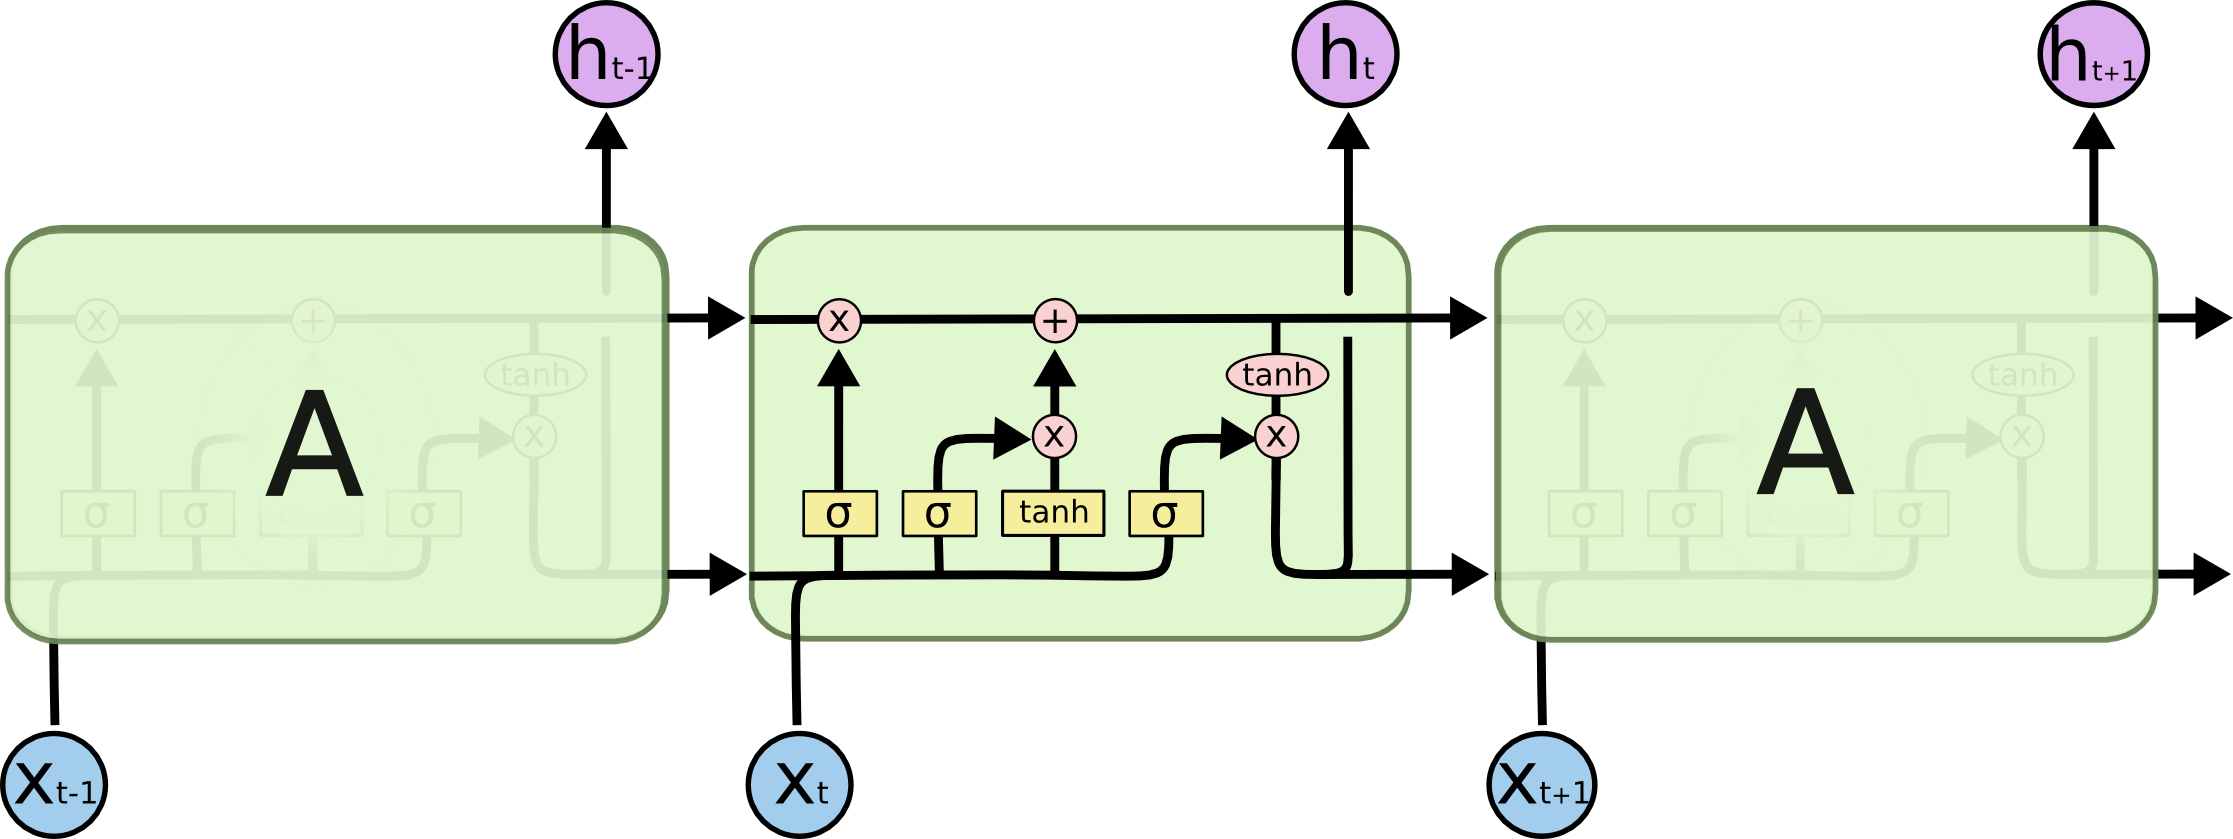
\includegraphics[width=35em]{lstm_02.png}

Sol ve sağdaki hücreler ortadakinin kopyası. 

Kıyasla bir RNN'nin iç yapısı çok daha basittir, 

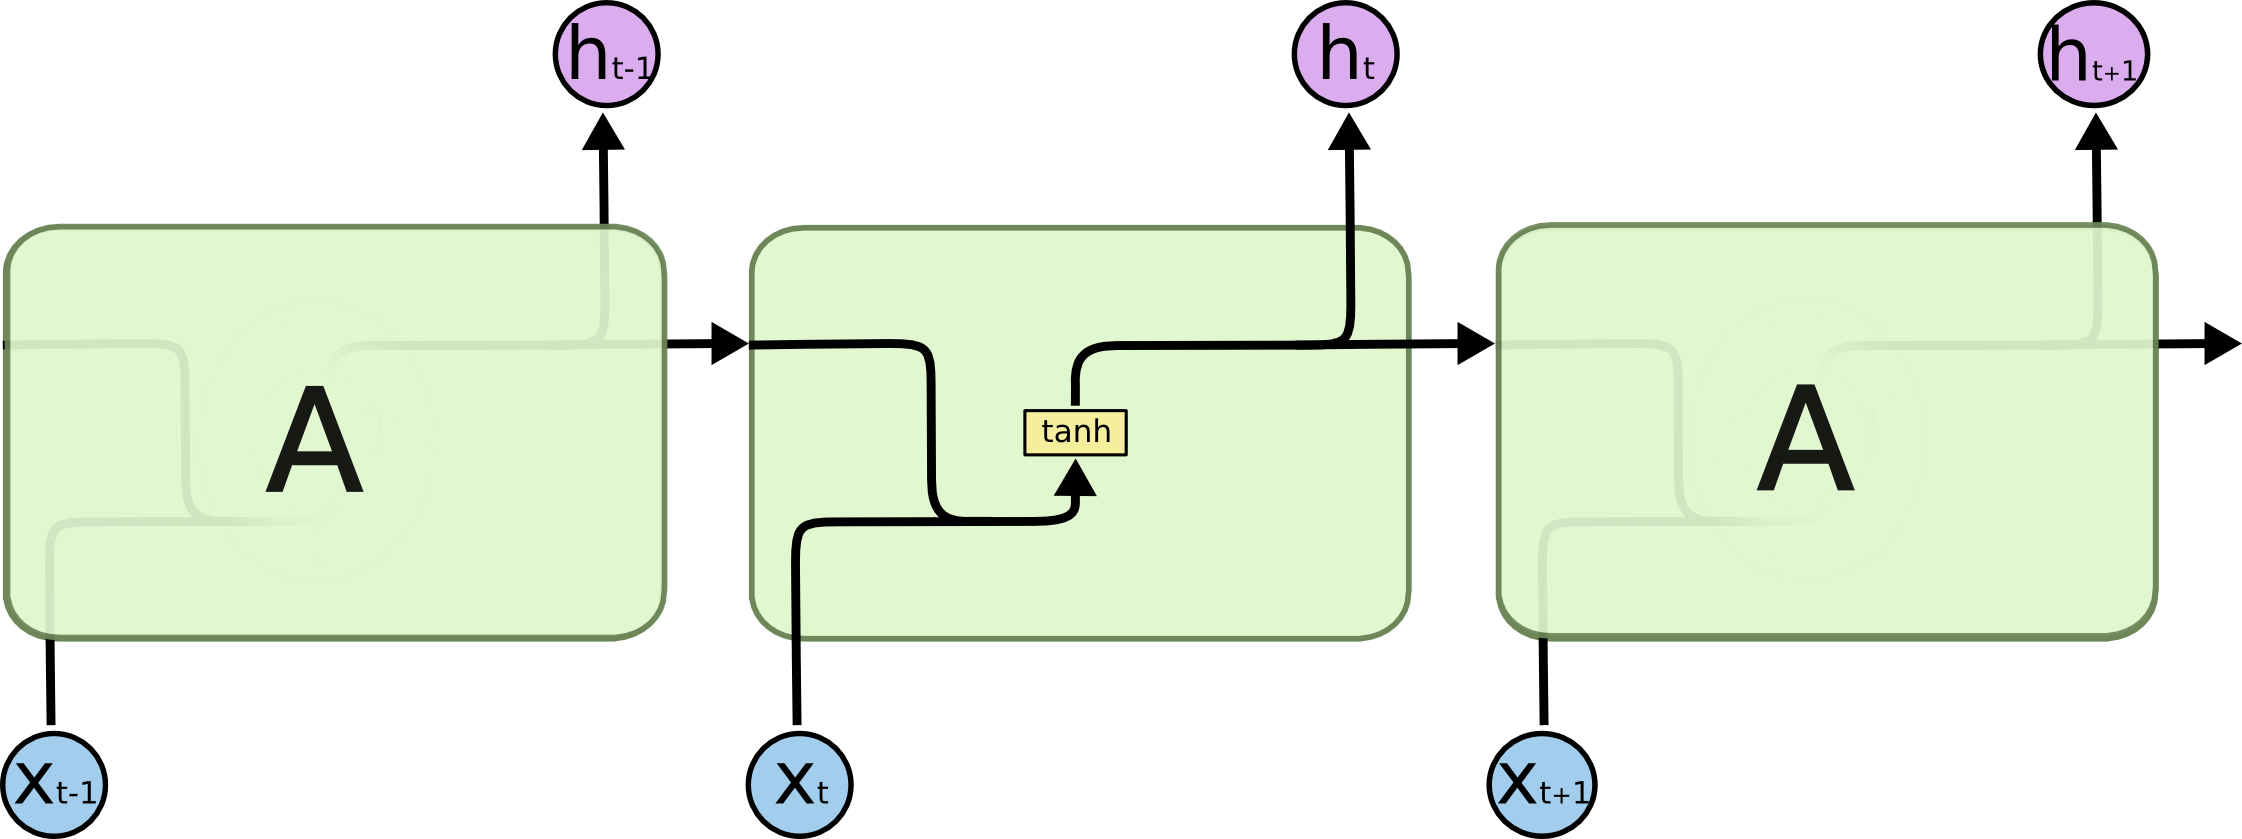
\includegraphics[width=35em]{lstm_03.png}

LSTM resmindeki her birimin formülleriyle beraber teker teker tekrar
üzerinden geçmek gerekirse [2] - ilk adım hücre bilgisinden neleri
atacağımıza karar vermek. Bu karar unutma karar tabakası adı verilen bir
sigmoid tabakasında veriliyor, tabaka $h_{t-1}$ ve $x_t$'ye bakıyor ve
$C_{t-1}$ hücre konumundaki her değer için 0 ile 1 arasında bir sayı
üretiyor. 1 değeri tamamen tut, 0 değeri tamamen unut anlamına geliyor (tüm
$b$ değerleri yanlılık -bias- için).

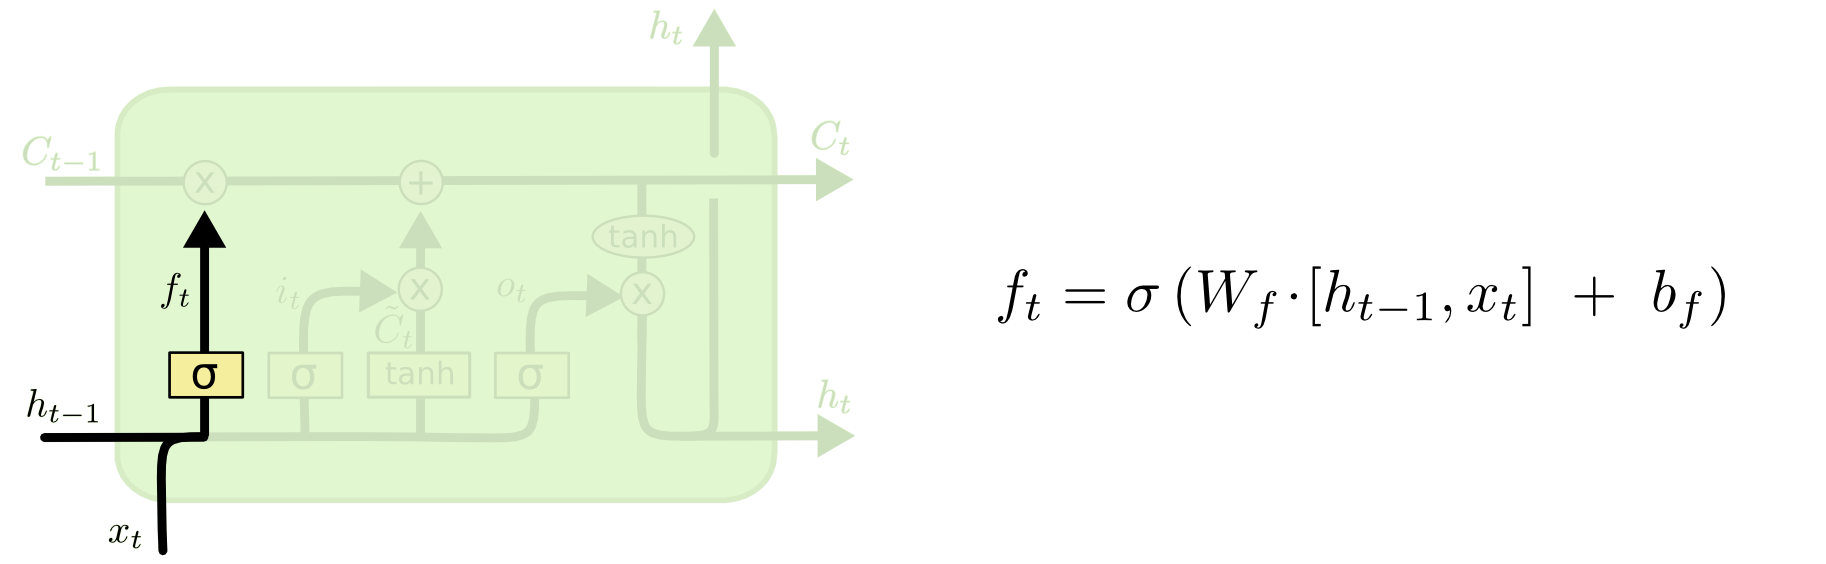
\includegraphics[width=35em]{lstm_04.png}

Bir sonraki adım hücrede hangi yeni bilgiyi depolayacağımıza karar
vermek. Bu kararın iki parçası var, önce girdi geçit tabakası (input gate
layer) hangi değerleri güncelleyeceğimize karar veriyor, ardından bir
$\tanh$ tabakası bir ``aday vektörü'' $\tilde{C}_t$ üretiyor, bu vektör,
adı üzerinde, hücre konumuna eklenmeye aday bilgiler. Ardından bu iki
vektör birleştirilip konumu güncellemek için yeni bir vektör yaratılıyor.

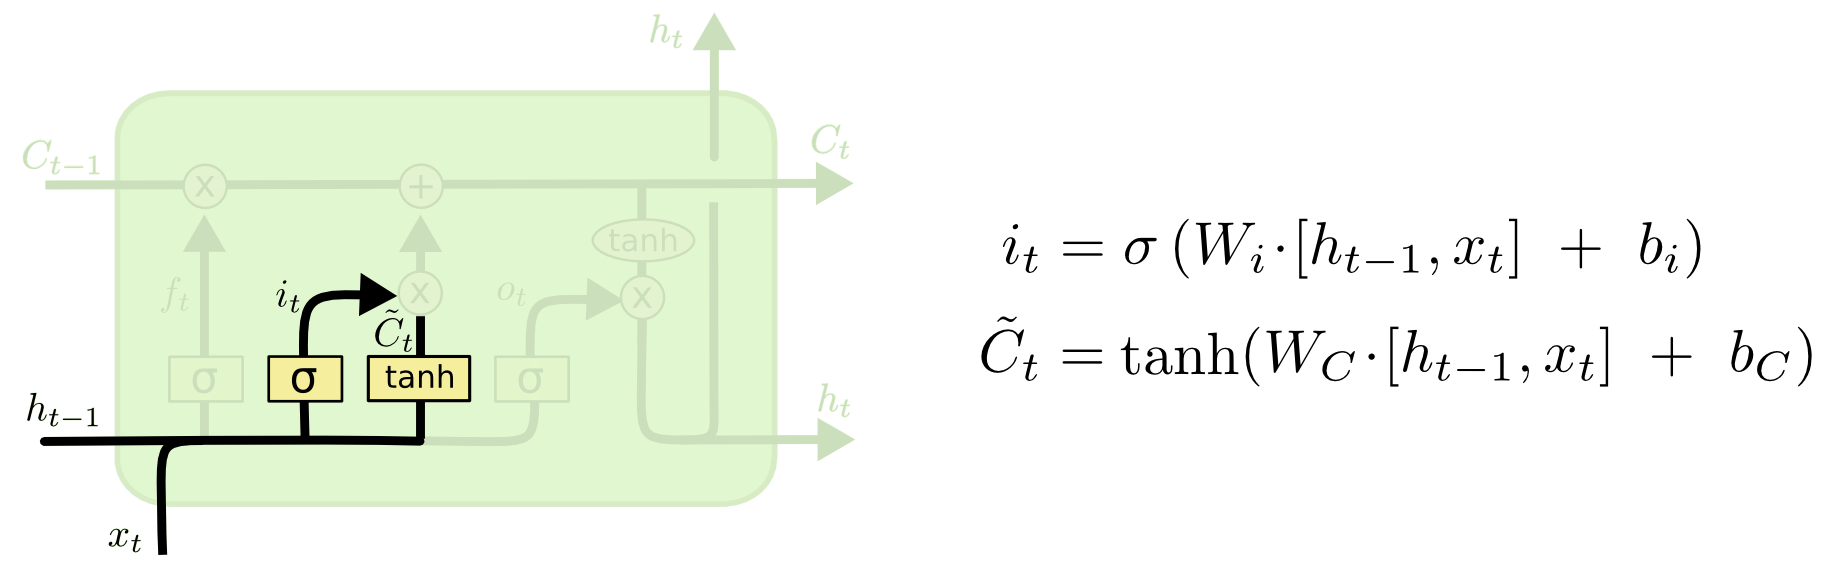
\includegraphics[width=35em]{lstm_05.png}

Sıra güncelleme iş bantına (update conveyor) geldi. Herhalde bu isim
verilmiş çünkü hücrenin en üstünde direk soldan sağa giden bu ok bir tür
fabrika iş bantı gibi, bir ana akım hattı. Bir kaç bilgi akımı bu ana kola
giriyor. Bu iş bantının görevi hücrenin eski konum bilgisini güncellemek,
$C_{t-1}$'i $C_t$ haline getirmek. Önceki adımlar ne yapılması gerektiğine
karar vermişti, şimdi bu kararları eyleme geçirme zamanı. Eski konum
bilgisini $f_t$ ile çarpıyoruz, böylece unutmak istediklerimizi
unutuyoruz. Sonra $i_t * C_t'$'yi ekliyoruz, bunlar yeni konumu ne kadar
güncellemek istediğimizi belirleyen ağırlıklarla ölçeklenmiş yeni aday
değerler.

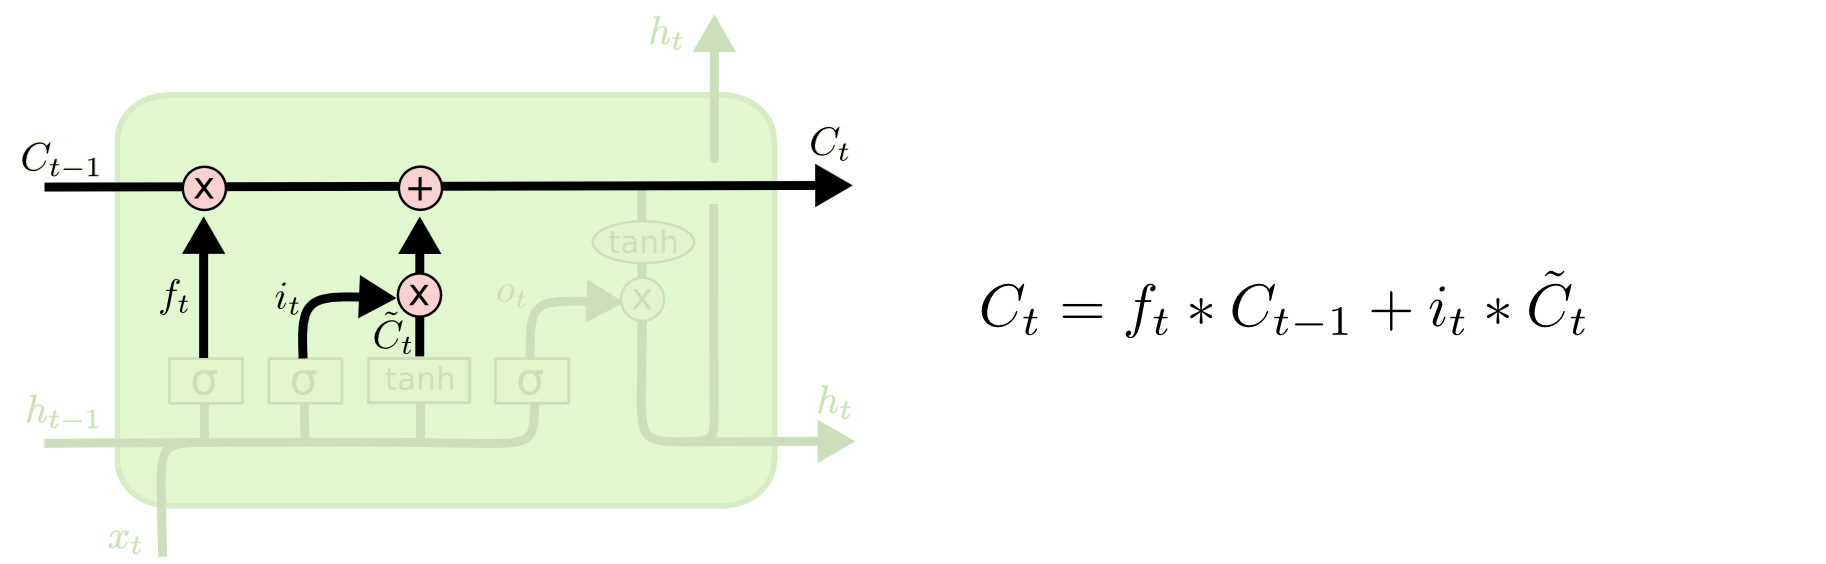
\includegraphics[width=35em]{lstm_06.png}

En son adım tahmin adımı, bu adımda artık çıktının ne olacağına karar
veriyoruz. Çıktı mevcut hücre konumunu baz alacak, ama onun filtrelenmiş
bir hali olacak. İlk önce bir sigmoid işleterek konumun hangi kısmının
çıktıya verileceğini kararlaştırıyoruz. Ardından mevcut konum bilgisini bir
$\tanh$'e veriyoruz, ki bu değerlerin $-1,+1$ arasında gelmesini
sağlıyoruz, ve bu sonucu sigmoid'den gelen değer ile çarpıyoruz, ki sadece
istediğimiz kısmın dışarı verilmesini sağlayalım. 

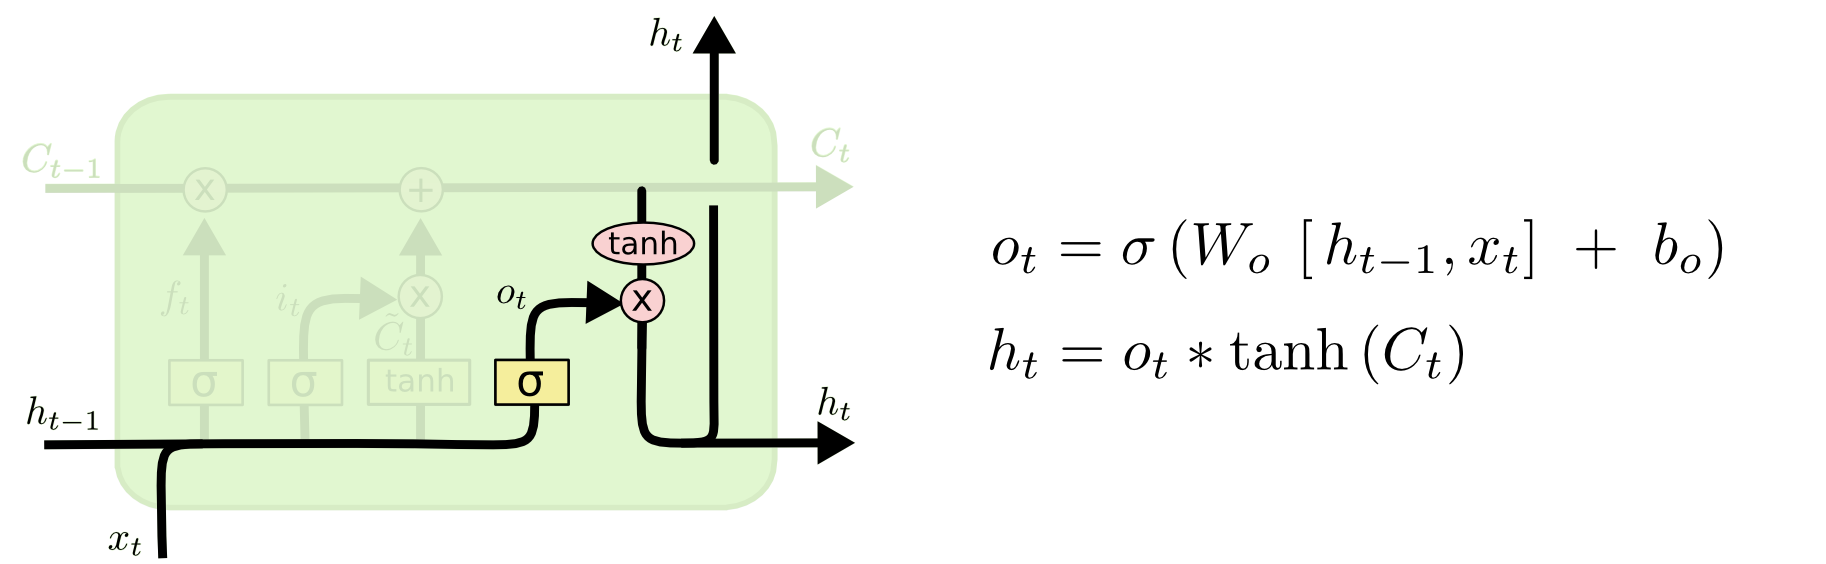
\includegraphics[width=35em]{lstm_07.png}

Şimdi üstteki formülleri kullanarak TensorFlow ile sıfırdan bir LSTM
kodlayalım. Amacımız daha önce RNN için gördüğümüz zaman serisini öğrenmek,
bu seriyi 5'er 5'er okuyacağız, yani yanyana 5 seri öğesini okuyacağız, ve
6. seri değeri hedef değeri olacak, seri içinden bu şekilde örneklem
yaparak bir ufak toptan eğitim seti yaratacağız. Sonra serinin hiç
görmediğimiz ``geleceğini'' tahmin etmeye uğraşacağız.

\begin{minted}[fontsize=\footnotesize]{python}
import tensorflow as tf
import numpy as np
from pprint import pprint
import datetime
import pandas as pd
import numpy as np
import matplotlib.pyplot as plt

tf.reset_default_graph()
np.random.seed(1)
tf.set_random_seed(1)

LSTM_SIZE = 30
t_min, t_max = 0, 30
resolution = 0.1
sequence_length = 4
instruction_count = 1
epoch = 500

def f(t):
    return t * np.sin(t) / 3 + 2 * np.sin(t*5)

def next_batch(batch_size, n_steps):
    t0 = np.random.rand(batch_size, 1) * (t_max - t_min - n_steps * resolution)
    Ts = t0 + np.arange(0., n_steps + 1) * resolution
    ys = f(Ts)
    X = ys[:, :-1].reshape(-1, n_steps, 1)
    y = ys[:, 1:].reshape(-1, n_steps, 1)
    y = y[:,-1,:]
    y = y.flatten()
    print y.shape    
    return list(X),y

reference_input_data,reference_output_data = next_batch(400, sequence_length)
   
# verinin 1/4'u egitim gerisi test
NUM_EXAMPLES = len(reference_input_data) / 4 
test_input = reference_input_data[NUM_EXAMPLES:]
test_output = reference_output_data[NUM_EXAMPLES:] 
train_input = reference_input_data[:NUM_EXAMPLES]
train_output = reference_output_data[:NUM_EXAMPLES]

print train_input[1]
print train_output[1]

data = tf.placeholder(tf.float32, 
                      [None, sequence_length, instruction_count], 
                      name='data')

target = tf.transpose(tf.placeholder(tf.float32, [None], name='target'))

FEATURE_SIZE = 1 

def default_weights_and_bias():
    Weights = tf.Variable(tf.truncated_normal([LSTM_SIZE, 
                                               LSTM_SIZE + FEATURE_SIZE], 
                                               -0.2, 0.1))
    bias = tf.Variable(tf.constant(0.0, shape = [LSTM_SIZE, 1]))
    
    return Weights, bias

W_f, _ = default_weights_and_bias()

b_f = tf.Variable(tf.constant(1.0, shape = [LSTM_SIZE, 1]))

# Unutma tabakasi
def f_t(ht_minus_1_and_xt):
    return tf.sigmoid(tf.matmul(W_f, ht_minus_1_and_xt) + b_f)

W_i, b_i = default_weights_and_bias()

# Girdi gecidi tabakasi
def i_t(ht_minus_1_and_xt):
    return tf.sigmoid(tf.matmul(W_i, ht_minus_1_and_xt) + b_i)

W_C, b_c = default_weights_and_bias()

# is banti icin adaylar
def candidate_C_t(ht_minus_1_and_xt):
    return tf.tanh(tf.matmul(W_C, ht_minus_1_and_xt) + b_c)

def C_t(ht_minus_1_and_xt, Conveyor, CandConv):
    return f_t(ht_minus_1_and_xt) * Conveyor + i_t(ht_minus_1_and_xt) * CandConv

W_o, b_o = default_weights_and_bias()

# guncellenmis is banti
def h_t(ht_minus_1_and_xt, FinalConveyor):
    o_t = tf.sigmoid(tf.matmul(W_o, ht_minus_1_and_xt) + b_o)    
    return o_t * tf.tanh(FinalConveyor)

def lstm_cell(ht_minus_1_and_Conveyor, xt):
    ht_minus_1, Conveyor = ht_minus_1_and_Conveyor
    
    ht_minus_1_and_xt = tf.transpose(tf.concat([ht_minus_1, xt], 1))
    
    CandidateConveyor = candidate_C_t(ht_minus_1_and_xt)
    
    FinalConveyor = C_t(ht_minus_1_and_xt, Conveyor, CandidateConveyor)
    
    lstm_prediction = tf.transpose(h_t(ht_minus_1_and_xt, FinalConveyor))
    
    return(lstm_prediction, FinalConveyor)

data_length = tf.shape(data)[0]

def lstm_loop(last_lstm_prediction, last_state, step):
    lstm_prediction, state = lstm_cell((last_lstm_prediction, last_state),
                                       data[:, step, :])
    return lstm_prediction, state, tf.add(step, 1)

initial_Conveyor = tf.zeros([LSTM_SIZE, data_length])

initial_prediction = tf.zeros([data_length, LSTM_SIZE])

timesteps = sequence_length

for_each_time_step = lambda a, b, step: tf.less(step, timesteps)

arg = (initial_prediction, initial_Conveyor, 0)
lstm_prediction, lstm_state, _ = tf.while_loop(for_each_time_step,
                                               lstm_loop, arg,
                                               parallel_iterations=32)

weight = tf.Variable(tf.truncated_normal([LSTM_SIZE, 1]))

bias = tf.Variable(tf.constant(0.0, shape=[1]))

prediction = tf.matmul(lstm_prediction, weight) + bias

with tf.name_scope('mean_square_error'):
    mean_square_error = tf.reduce_sum(tf.square(tf.subtract(target, tf.unstack(prediction, axis = 1))))
    
tf.summary.scalar('mean_square_error', mean_square_error)

optimizer = tf.train.AdamOptimizer()

minimize = optimizer.minimize(mean_square_error)

mistakes = tf.not_equal(target, tf.round(tf.unstack(prediction, axis = 1)))

sess = tf.InteractiveSession()

date = str(datetime.datetime.now())

init_op = tf.global_variables_initializer()

saver = tf.train.Saver() 

sess.run(init_op)

for i in range(epoch):
    if (i + 1) % 20 == 0:
        mean_squ_err = sess.run(mean_square_error, {data: test_input, target: test_output})
        print('Epoch {:4d} | mean squ error {: 3.1f}'.format(i + 1, mean_squ_err))
    
    sess.run(minimize,{data: train_input, target: train_output})
\end{minted}

\begin{verbatim}
(400,)
[[ 4.00159218]
 [ 4.4298434 ]
 [ 4.67217731]
 [ 4.52697138]]
3.87853505042
Epoch   20 | mean squ error  3181.8
Epoch   40 | mean squ error  1860.6
Epoch   60 | mean squ error  1307.7
Epoch   80 | mean squ error  903.1
Epoch  100 | mean squ error  628.8
Epoch  120 | mean squ error  477.8
Epoch  140 | mean squ error  390.5
Epoch  160 | mean squ error  323.5
Epoch  180 | mean squ error  271.9
Epoch  200 | mean squ error  233.8
Epoch  220 | mean squ error  204.4
Epoch  240 | mean squ error  180.8
Epoch  260 | mean squ error  161.2
Epoch  280 | mean squ error  144.9
Epoch  300 | mean squ error  131.7
Epoch  320 | mean squ error  121.4
Epoch  340 | mean squ error  113.0
Epoch  360 | mean squ error  105.7
Epoch  380 | mean squ error  99.0
Epoch  400 | mean squ error  92.6
Epoch  420 | mean squ error  86.6
Epoch  440 | mean squ error  80.9
Epoch  460 | mean squ error  75.4
Epoch  480 | mean squ error  70.1
Epoch  500 | mean squ error  64.9
\end{verbatim}

Tahminleri üretirken eğitim verisinin en sonundaki \verb!sequence_length!
kadar öğeyi alıp sonraki 1 değeri üretiyoruz, bu değeri alıp tahmin için
kullanılan biraz önce kullandığımız \verb!sequence_length! kadar değerin
sonuna ekleyip son \verb!sequence_length! değer üzerinden tekrar bir
tahmin üretiyoruz, böyle gidiyor, ve bu şekilde serinin hiç görmediğimiz
kısmını tahmin ediyoruz.

\begin{minted}[fontsize=\footnotesize]{python}
def f(t):
    return t * np.sin(t) / 3 + 2 * np.sin(t*5)

t = np.linspace(t_min, t_max, int((t_max - t_min) / resolution))
y = f(t)

newx = list(t[-sequence_length:])
newy = list(y[-sequence_length:])

for i in range(40): # bu kadar daha uret
   tst_input = np.array(newy[-sequence_length:]).reshape(sequence_length,1)   
   res = sess.run(prediction, { data: [ tst_input ]  } )
   newy.append(res)
   newx.append(t_max + (i*resolution))

plt.plot(t,y)
plt.plot(newx,newy,'g')
plt.savefig('lstm_01.png')
\end{minted}

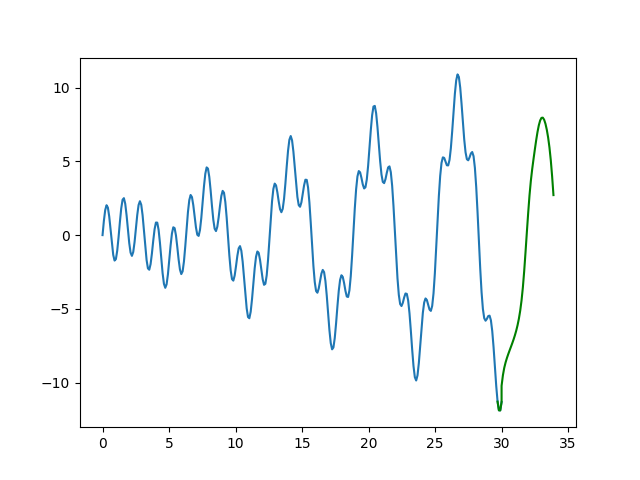
\includegraphics[width=20em]{lstm_01.png}

Yeşil renkli kısım tahmin. Fena değil.

Zaman Serisi Sınıflandırmak

Şimdi TF'in kendi LSTM çağrısını kullanarak zaman serisi sınıflandırması
yapalım. İki farklı sınıfa ait olan zaman serisi verimiz var [3],
mikroelektronik yarı-iletken üretiminden gelen bir veri, fabrikasyon
sırasında algılayıcılar bu iki türlü seriyi kaydediyor, onları ayırtetmek
bizim görevimiz. Okuma yöntemi kodlayalım,

\begin{minted}[fontsize=\footnotesize]{python}
import pandas as pd, zipfile
import tensorflow as tf
from tensorflow.contrib import rnn

learning_rate = 0.001
training_iters = 100000
batch_size = 25
display_step = 10

n_input = 1 
n_steps = 152 
n_hidden = 128 
n_classes = 2

with zipfile.ZipFile('wafer.zip', 'r') as z:
      df_train =  pd.read_csv(z.open('Wafer/wafer_TRAIN.txt'),header=None)
      df_test =  pd.read_csv(z.open('Wafer/wafer_TEST.txt'),header=None)

def minibatches(batch_size,input="train"):
      df = None
      if input=="train": df=df_train
      if input=="test": df=df_test
      df = np.array(df)
      for i in range(len(df)):
            batch_x = []; batch_y = []
            for j in range(batch_size):
                  batch_x.append(list(df[i,1:]))
                  batch_y.append([int(df[i,0]==-1), int(df[i,0]==1) ])
            batch_x = np.array(batch_x).reshape(batch_size,n_steps,1)
            batch_y = np.array(batch_y).reshape(batch_size,2)
            yield batch_x, batch_y                  

\end{minted}

TF hesap çizitini kodlayalım ve eğitelim,

\begin{minted}[fontsize=\footnotesize]{python}
def reset_graph(seed=42):
    tf.reset_default_graph()
    tf.set_random_seed(seed)
    np.random.seed(seed)

reset_graph()

x = tf.placeholder("float", [None, n_steps, n_input])
y = tf.placeholder("float", [None, n_classes])

weights = {
    'out': tf.Variable(tf.random_normal([n_hidden, n_classes]))
}
biases = {
    'out': tf.Variable(tf.random_normal([n_classes]))
}

def LSTM(x, weights, biases):
    x = tf.unstack(x, n_steps, 1)
    lstm_cell = rnn.BasicLSTMCell(n_hidden)
    outputs, states = rnn.static_rnn(lstm_cell, x, dtype=tf.float32)
    return tf.matmul(outputs[-1], weights['out']) + biases['out']

pred = LSTM(x, weights, biases)

correct_pred = tf.equal(tf.argmax(pred,1), tf.argmax(y,1))
accuracy = tf.reduce_mean(tf.cast(correct_pred, tf.float32))
new_pred = tf.argmax(y,1)

print 'cost'
scf = tf.nn.softmax_cross_entropy_with_logits(logits=pred, labels=y)
cost = tf.reduce_mean(scf)
print 'optimizer'
optimizer = tf.train.AdamOptimizer(learning_rate=learning_rate).minimize(cost)

init = tf.global_variables_initializer()

with tf.Session() as sess:
    sess.run(init)
    step = 1
    # Keep training until reach max iterations
    b_it = minibatches(batch_size)
    while step < int(1000 / batch_size):
          batch_x, batch_y = next(b_it)
          sess.run(optimizer, feed_dict={x: batch_x, y: batch_y})
          if step % display_step == 0:
                # Calculate batch accuracy
                acc = sess.run(accuracy, feed_dict={x: batch_x, y: batch_y})
                # Calculate batch loss
                loss = sess.run(cost, feed_dict={x: batch_x, y: batch_y})
                print("Iter " + str(step) + ", Minibatch Loss= " + \
                      "{:.6f}".format(loss) + ", Training Accuracy= " + \
                      "{:.5f}".format(acc))
          step += 1

    print("Optimization Finished!")
\end{minted}

\begin{verbatim}
cost
optimizer
Iter 10, Minibatch Loss= 1.847300, Training Accuracy= 0.00000
Iter 20, Minibatch Loss= 0.049264, Training Accuracy= 1.00000
Iter 30, Minibatch Loss= 0.176535, Training Accuracy= 1.00000
Optimization Finished!
\end{verbatim}

\begin{minted}[fontsize=\footnotesize]{python}
saver = tf.train.Saver()
from sklearn import metrics
real = []
pred = []
with tf.Session() as sess:
    for batch_x, batch_y in minibatches(1,input="test"):
      res = sess.run(new_pred, feed_dict={x: batch_x, y: batch_y})
      pred.append(res[0])
      real.append(np.argmax(batch_y[0]))
    fpr, tpr, thresholds = metrics.roc_curve(np.array(real), np.array(pred))
    print 'AUC', metrics.auc(fpr, tpr)      
\end{minted}                    

\begin{verbatim}
AUC 1.0
\end{verbatim}

Sonuç yüzde 100. 

Kaynaklar

[1] Chen, {\em Exploring LSTMs: Understanding Basics (Part One)}, \url{https://www.topbots.com/exploring-lstm-tutorial-part-1-recurrent-neural-network-deep-learning/}

[2] Shell, {\em Do It Yourself LSTM with TensorFlow}, \url{https://chrisschell.de/2017/07/10/do_it_yourself_lstm_with_tensorflow.html}

[3] Olszewski, {\em Wafer Dataset}, \url{http://timeseriesclassification.com/description.php?Dataset=Wafer}

[4] Olah, {\em Understanding LSTM Networks}, \url{https://colah.github.io/posts/2015-08-Understanding-LSTMs}

\end{document}

